\documentclass[a4paper,11pt]{article}

\usepackage[english]{babel}
\usepackage[utf8x]{inputenc}
\usepackage{amsmath}
\usepackage{graphicx}
\usepackage[margin=0.5in]{geometry}
\usepackage{caption}
\usepackage{subcaption}


\begin{document}

{\Huge Time Series Causality Algorithm (TSC1) Notes}
(
\hfill\rule{150mm}{.1pt}

\hfill{\small \today}

\section{Example 1}
Consider a block sliding down a frictionless ramp.  The system is assumed to be conservative, so
$$
\frac{mv^2}{2} = mgh = mg d\sin\theta = mg vt\sin^2 \theta
$$
where $v$ is the velocity of the block, $t$ is the time the block has been in motion, $m$ is the mass of the block, $g$ is the local acceleration due to gravity, $h$ is the height of the block before it is released, and $d$ is the distance the block has traveled.  The velocity is then  
$$
v(t) = 2gt\sin^2 \theta\;\;.
$$
If the angle of the ramp is varied with time as
$$
\theta(t) = \sin(t)\;\;,
$$
then it is expected that $\theta(t)\rightarrow v(t)$, i.e.\ the changing angle drives the changing magnitude of the velocity.

The angle driving signal and the velocity response signal are seen in Figure \ref{fig:thetaandv}.
\begin{figure}[ht]
\begin{tabular}{ll}
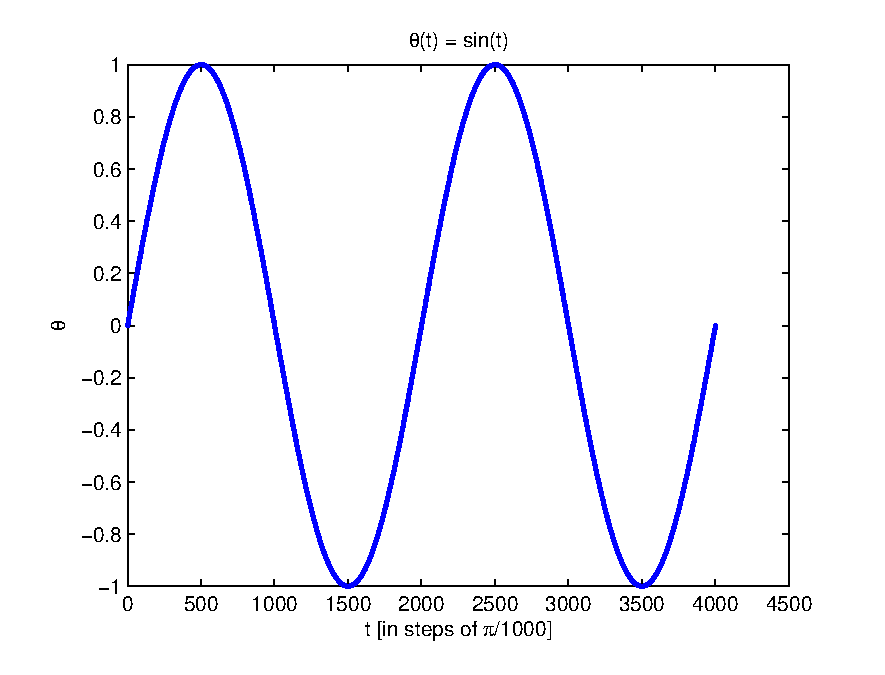
\includegraphics[scale=0.65]{theta.eps} & 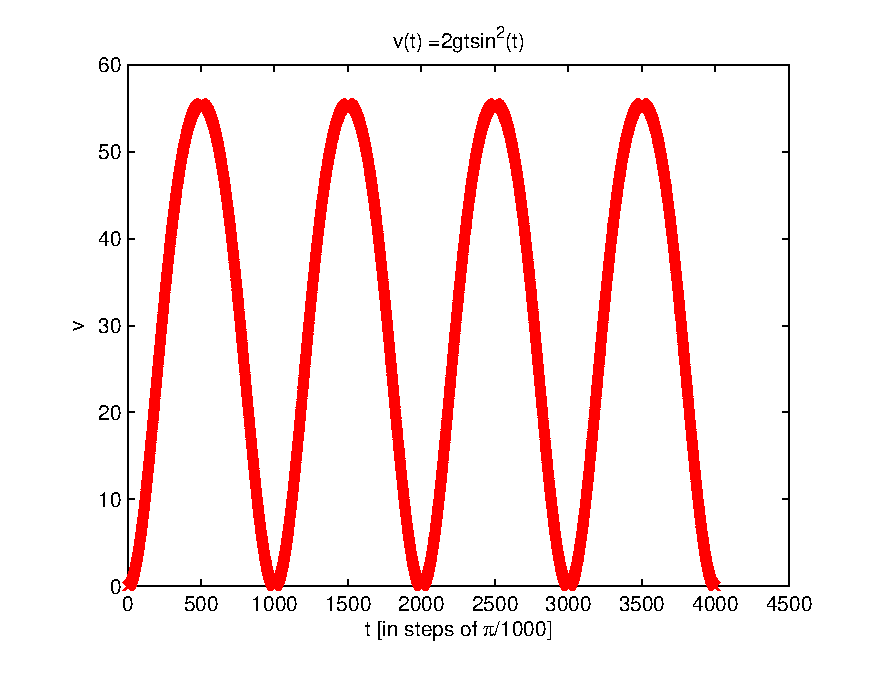
\includegraphics[scale=0.65]{v.eps}\\
\end{tabular}
\caption{}
\label{fig:thetaandv}
\end{figure}

The change in $\theta$ is expected to affect $v$, so a first step is to find the distribution of changes in $\theta$; i.e.\
$$
\delta\theta(t) \equiv \frac{d\theta}{dt} \approx \frac{\Delta\theta}{\Delta t} = \theta(t)-\theta(t-1)\;\;.
$$
A histogram of $\{\delta\theta(t)\;|\;t\ge 0\}$ is seen in Figure \ref{fig:dthetahist}.
\begin{figure}[ht]
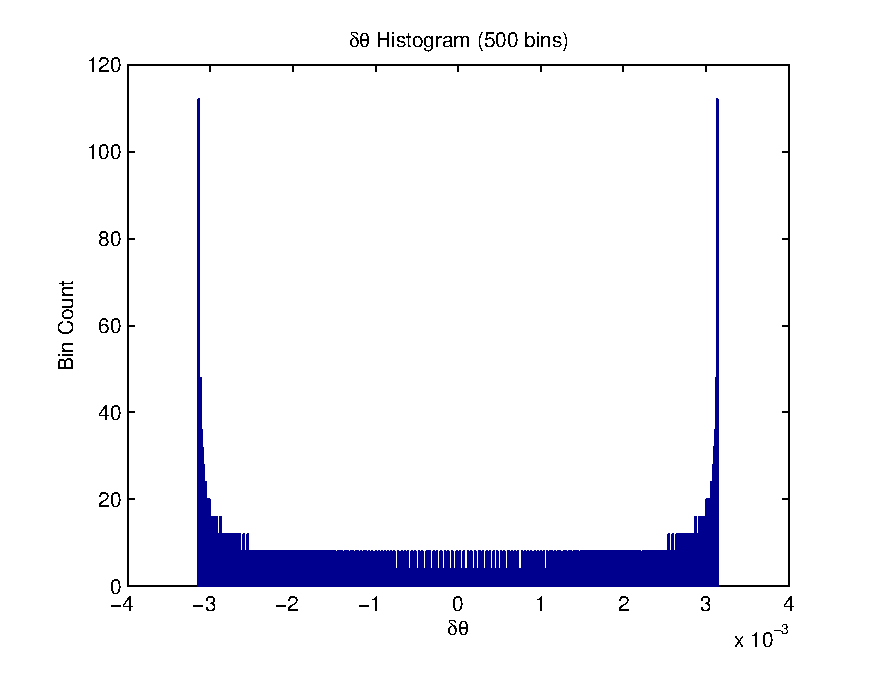
\includegraphics[scale=0.65]{dthetahist.eps}
\caption{}
\label{fig:dthetahist}
\end{figure}
A given bin can be picked (e.g.\ bin 125 in Figure \ref{fig:dthetahist}), and the values of $v$ that occur immediately following the binned $\delta\theta$ can be plotted to give an idea of how the response signal reacts to the given change in the driving signal.  Let $B_i = \{t_k\}$ be the set of times $t$ corresponding to the $i$th bin of $\delta\theta$ which contains all the $\{\delta\theta(t_k)\}$ that belong to that bin.  The plot of the correspondingly binned response signal would be a plot of $\{v(t+1)\;|\; t\in B_i\}$.  Figure \ref{fig:vbin125} is such a plot for $B_{125}$.
\begin{figure}[ht]
\includegraphics[scale=0.65]{vbin125.eps}
\caption{}
\label{fig:vbin125}
\end{figure}

Conceptually, the response signal is expected to have only a few different values in response to a given change in the driver.  However, it might be expected that the actual value of the response might also depend on the previous value of the response signal.  For example, a $0.25\pi$ change in $\theta$ would lead to a different value of $v(t)$ depending on $v(t-1)$.  Two ways to approach this problem are to define a change in $v$ (i.e.\ $\delta v$) and then investigate $\{\delta v(t+1)\;|\; t\in B_i\}$ or to bin $v$ and then investigate $\delta\theta$-binned response values $v$ within a given $v$-binned set.  Both methods are explored below.

\subsection{$\delta\theta$ leads to $\delta v(t)$}
The set $\{\delta\theta(t_k)\;\forall t_k\in B_i\}$ can be compared with $\{\delta v(t_k+1)\}$ to understand how similar changes in $\theta$ are followed by changes in $v$.  Figure \ref{fig:dthetadv} shows such a plot for $i=125$.
\begin{figure}[ht]
\begin{tabular}{ll}
\includegraphics[scale=0.65]{dthetabin125.eps} & \includegraphics[scale=0.65]{dvbin125.eps}\\
\end{tabular}
\caption{}
\label{fig:dthetadv}
\end{figure}
The figures show that for $B_{125}$ two separate values of $\delta v(t_k+1)$ seem to follow $\delta\theta(t_k)$, implying
$$
\delta\theta(t_k) = 
$$

\end{document}